

\chapter{Planning}

\label{Chapter4}

In this section I will talk about some of the things I have done to make sure everything goes as planned and my time is used efficiently. 

\section{Gantt chart}
Gantt charts are a nice way to keep track of your time available over a whole project. It really helps understand the scope of things and to give a better estimate on how to split up your time into smaller chunks.
\begin{figure}[!h]
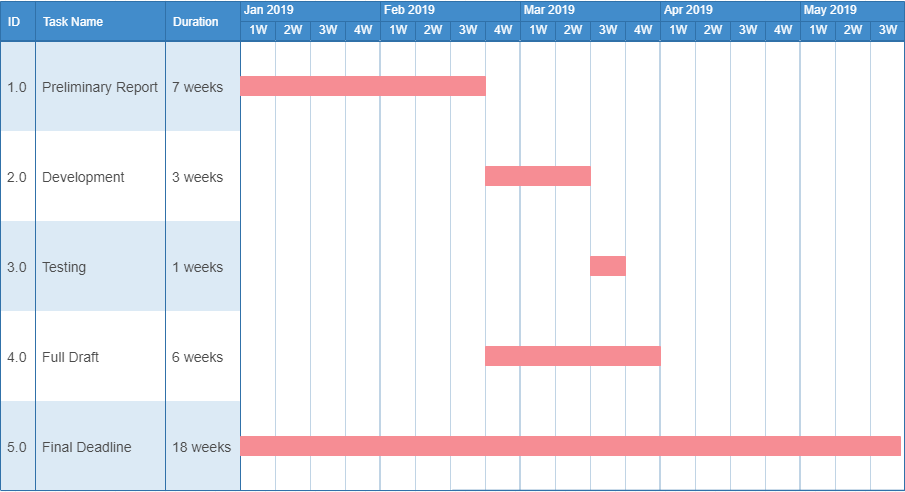
\includegraphics[width=150mm]{figures/gantt_chart}
\caption{Gantt chart}
\end{figure}

Here you can see the gantt chart created for this project. It has a rough sketch of the bigger tasks, nothing too precise, as it is helpful enough this way to keep track of the weeks overall.

\section{Progress Logs}
The weekly progress logs act as a weekly sprint. In them I write down what I did, what I wanted to do and what I will do by next week. This helps keep track of the more short term week-by-week goals. I also find the recaps at the end of the week to be quite helpful to remind myself of what I did and what I still need to do. 

\section{Version Control}
Version control is an essential part of any project. I'm using GitHub, but there are many others out there that do the same job. It helps mainly because of the ability to go back to previous versions whenever needed, for example when something goes horribly wrong. 
\begin{figure}[!h]
	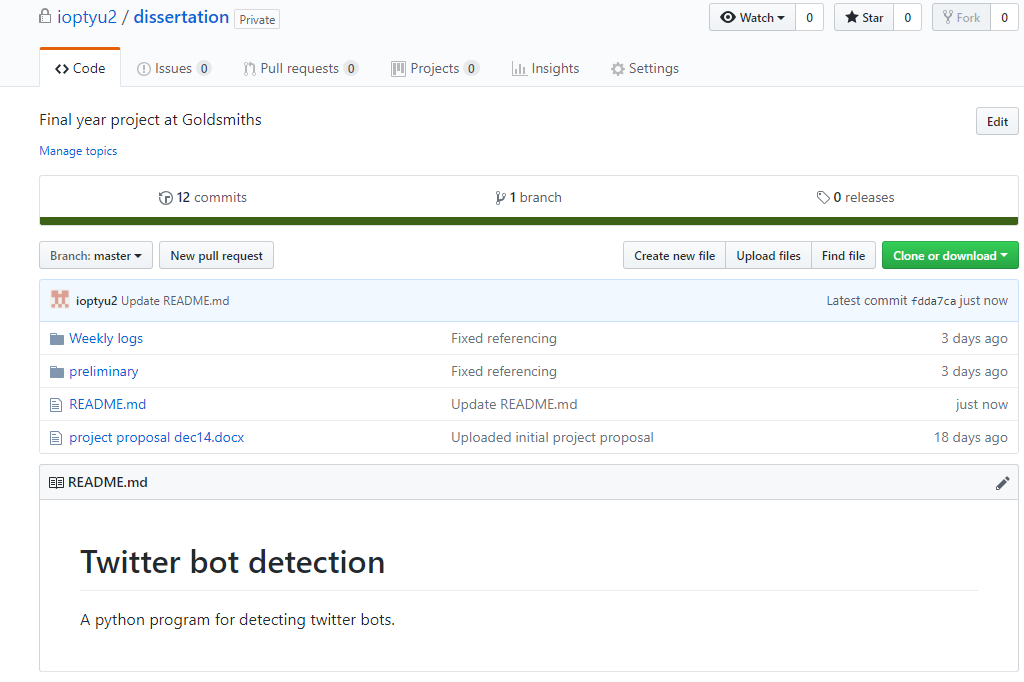
\includegraphics[width=140mm]{figures/github}
	\caption{Github Repository}
\end{figure}
